\chapter{Analysis}
\label{analysis}

\lettrine[lraise=0.1, nindent=0em, slope=-.5em]{\color{Violet}T}{his} chapter provides analytical part of the thesis beginning with analysis of the current situation following with analysis of the problems. Thereafter a requirement list for new e-course being established, followed by decision for methodology chosen for development of the e-course. 

\section{Problem Analysis}
\label{Problem Analysis}


Deficit of skilled \gls{ICT} specialist are known problem in Estonia \citep{website:ict_puudu} \citep{website:ict_needs}. However, several higher education institutes increased number of spots in \gls{ICT} curricula the outcome is insufficient \citep{website:TU_ict}, \citep{website:itc_facts}. Moreover, continuous changing and continuous learning are common in \gls{ICT} field. Therefore, a development of \gls{ICT} curriculum are continual activities in \gls{EITC} to maintain professionalism as a specialist.

During curriculum development process the \gls{EISA} contacted with \gls{EITC} describing a problem: The deficiency of the skilled and security aware system administrators and also provide initial proposal for solution as seen in Appendix~\ref{Letter from CERT.EE to the Rector of Estonian IT College} on page ~\pageref{Letter from CERT.EE to the Rector of Estonian IT College}. However, instead of accepting the solution without questioning we arranged several workshops for initial investigation of the problem and divided it to separate sub-problems and suggestions. For ensuring wider view of the problem several experts where involved from private companies, telecoms, banks, small business and start-ups.

First, many system administrators acquired their knowledge through self-study. However, a continuous study is common in \gls{ICT} field the level of the specialist are unsteady and they do not have sufficient knowledge to build secure infrastructure.

Second, the applied education field do not provide needed qualification needed to manage secure it infrastructure services.

Third, in retraining field is usual that private companies offer several courses for configuring and securing infrastructure, networks and services. However, those trainings are usually vendor based and focused heavily for promoting proprietary technologies.

Fourth, the system administrators in local government or municipal field constitute a whole with unevenly level of skills and knowledge. Therefore making maintaining and helping of the target group difficult for \gls{CERT.EE}.


Fifth, all courses (needed to be developed) should be associated with the practical applicability of the theoretical knowledge and contain largely practical hands-on classes. Moreover, all materials should be based on not proprietary technology, like \gls{OpenBSD} or \gls{GNU/Linux}.

Sixth, the study program should focuses on practical learning by doing approach to \gls{ICT} subjects. Moreover, using virtual and game-like environments is a contemporary approach for teaching IT System administration and programming focusing to the cyber security requirements increases a motivation of students. Today the studies include lectures, practical classes and independent work as homework. By and large, one subject is divided as follows: 25\% lectures, 25\% practical classes and 50\% homework which is mostly working with materials (books, web articles). In the worst case, practical work constitutes only 25\% and takes place at \gls{EITC} computer classes.
Moreover, the students are not interested in learning mere theory. The formulas are not seen necessary nor linked to their study area or future job. Theory that is not used will be forgotten quickly. In a few years students won't even remember if a specific topic was covered or not. Applied education should introduce practical approach and learning by doing. In ITC field practical classes and practical homework is the key to achieving acceptable results.
In initial investigation phase the authors role was curricula development, requirements management,  planning hands-on labs and course descriptions.


Designing an e-course is a challenge that has been solved by many lecturers and instructional developers. Moreover, the popularity of the cyber security related subjects in information and communications technology ICT curricula is growing and become a "student’s magnet" for higher educational institutes \citep{CyberIsHot}. Thereafter is possible to gain additional information by analysing related curricula in several higher educational institutes and analysing instructional design methodologies to achieve goals of this thesis.

\section{Related Work}
\label{Related Work}
Related Work...
ONE PAGE MAX
Panna siia lühikokkuvõte loetud teadusartikklitest IEEE*

Kauri magistritöö

Antud probleem pole maailmas unikaalne. Sama probleemi on lahendanud XXX tööd. Antud töö on veidi erinev enamlevinud lahendustest, kuna keskendub kaitse õpetamisele. Lisaks võetakse arvesse lokaaseid tingimusi ja sithgruppi. Need kaks komponenti moodustavad töö uudsuse.

Võib jagada kursusteks ja ülesanneteks.

Võtame kasutusele eelmistest töödest õpitu:
Kasak Kaur \citep{KasakKaur}
Competition between students...
Capture the flag ei toimi ... kui just flag ei ole info, mis identifitseerib ründaja...

Kursused:

Meelis Roos turvaline programmeerimine
Meelis Roos turve 

OWASP materjalid - Head ja sobivad kasutada!

Jätame välja NFS, NIS unsecure LDAP jne ründed.
Samuti jätame välja password crackingu. pigen nõuame, et rakendataks OS PAM password policyt + cracklibi.


\section{Choosing Methodology for Developing an e-course}

Developing a course instructions can proceeded using several methodologies. However, before choosing suitable approach for practical cyber security course some explanation of the terms e-course, e-learning, learning object, blended learning and hands-on laboratory classes are given to establish clear understanding for terminology used in thesis.

The term E-learning can be defined as the use of computer and Internet technologies to deliver a broad array of solutions to enable learning and improve performance \cite[p.~3]{food2011learning}.
V. Waller and J. Wilson 
E-course is a e-learning course and can be divided to one or several learning objects - {\color{red} TODO }

Learning object -  as a part of \gls{e-course} {\color{red} TODO }

Blended learning - {\color{red} TODO }

Hands-on laboratory - {\color{red} TODO }

Instructional design - {\color{red} TODO }

Today a learning by doing approach is accepted way to gain new skills and knowledge in cyber security field. This thesis focuses to develop of the practical hands-on e-course for system administrators in \gls{EITC}. Moreover the developed laboratories are used in higher education and also in continuous education classes.



\url{http://www.createdebate.com/debate/show/How_relevant_is_the_ADDIE_model_in_2009}

ADDIE model \url{http://www.youtube.com/watch?v=fdpHO1xycgo&list=PLEBAA915299F438EB}


Haridustehnoloogia sõnastik - \url{http://wiki.e-uni.ee/htsonastik/index.php?n=Main.Otilde#oppematerjal}

Miks creative common - \url{http://www.copyrightreform.eu/case-for-copyright-reform}

Alternative Training Models
Advances in Developing Human Resources November 2006 8: 460-475,


The methodology used to develop this e-course should encourage student activity in learning process. Moreover student should have possibility to choice learning speed, -place and -time. Today's students have different learning style and background and methodology should reckon with individual differences...

Developed e-course should support people with disabilities. In \gls{EITC} several people have hearing disabilities and all important material should presented also without audio. For example in screen casts videos all important information should be written also in screen or added as transcript.

Today’s learning environment should support student communities where students can act as mentors and also feel part on the study program. Course integration with student driven initiative like forums, blogs, wiki pages and other collaboration learning methods should be possible and not restricted.


Developing an e-course can be done without using design methodology but systematic approach should give more effective results. In principle the common systematic methods to develop an e-learning course are applying a Instructional System Design \gls{ISD} (sometimes cited as  Instructional Design \gls{ID}) model. However, several \gls{ISD} modes exists and can divided into three classes: behaviorism, cognitivist and prescriptive design \citep{website:id_models}, this thesis uses Prescriptive Design Model and specifically the \gls{ADDIE} process because method is used in Estonia and recommended for designing e-learning course \citep[p.~5]{OppeArenduskeskus2010}. Moreover, the \gls{ADDIE} model is not only good model that can be customized to meet specific needs, but ADDIE is a commonly used effective model for instructional  design \citep{ieee_addie_1607206}.


 However, the \gls{ADDIE} model has several weaknesses as \url{http://www.instructionaldesign.org/models/index.html}
Although the ADDIE model is not modelling anything and technically should it called \gls{ID} framework \citep{bichelmeyer2004addie}, in this thesis term ADDIE model is used because this name is commonly known and used for designing e-learning courses \citep{bichelmeyer2004addie, OppeArenduskeskus2010}.
For conclusion the \gls{ADDIE} model was chosen to develop cyber security e-learning course and model is described in the next section.

\subsection{The ADDIE Model}

The \gls{ADDIE} model is used for creating different types of instructions as courses, trainings \citep{website:addie, lohr1998using}. Moreover, the ADDIE method is  used to provide a systematic, iterative course development process with feedback-based approach to improve quality of study \citep{website:using_addie}.

The ADDIE model contain five stages: Analysis, Desing, Development, Implementation and Evaluation as seen in illustration~\ref{figure:the addie model} \citep{website:addie}



\begin{figure}
 \centering 
 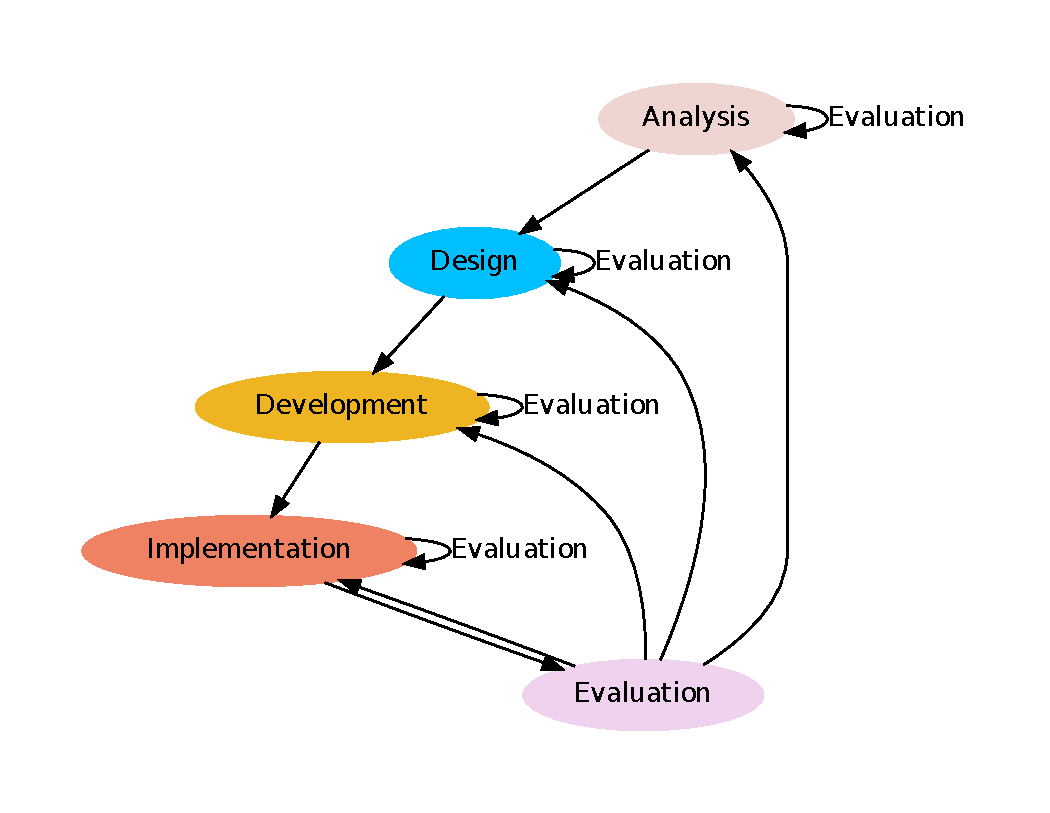
\includegraphics[width=0.6\textwidth]{addie_model.pdf}
 \rule{35em}{0.5pt} 
 \caption{The ADDIE model} 
 \label{figure:the addie model} 
\end{figure}

Firstly, the goal of the analysis phase is for investigation of the gap between goal and
existing situation. Therefore, this phase investigates instructional goals, current situation, learner, objectives \citep{chen2007learning, website:addie}.

Secondly, the design phase focuses following areas; assessments design, learning content, learning strategies and course format \citep{chen2007learning, website:addie}.


Thirdly, the work of development includes creating of course materials, choosing methodology and technologies, testing of material using run-through with small group. \citep{OppeArenduskeskus2010, website:addie, chen2007learning}.


Fourthly, the implementation stage is describes implementing the above work of three previous steps and gives possibility to evaluate full course in evaluation phase \citep{chen2007learning, website:addie}.


Finally, the evaluation phase is for assessing of the learning effect through evaluation. However the evaluation process takes place in every stage as seen in illustration~\ref{figure:the addie model} the final evaluation focuses whole course and focuses to the feedback from students and lecturers and output of this phase is valuable for next courses \citep{OppeArenduskeskus2010, website:addie}.



\section{Cyber security aspects of the e-learning}
Before starting instructional analysis of the e-learning course the cyber security aspect needs investigation to corrections and local modifications to the course development process. Therefore some questions need answer: Firstly, how studing cyber security affects student behaviour for example using learned methodologies to attack live systems? Secondly, does teaching in this field require special equipment comparing usual study of system administration? Thirdly, does field affect an usage of the methodology \gls{ADDIE} model chosen?

{\color{red} Uurida erinevaid cyber kursuseid } 


\section{Analysis of the e-learning course}
According to \gls{ADDIE} model the analysis stage establishes goals for the course and evaluation of the current situation and strategy for implementing goals followed by analysis of the learners and the content of the course \citep{website:addie}

The analysis phase of the \gls{ADDIE} model contains four sub-phases \citep{website:addie}.
\begin{enumerate}
\item Instructional Goals -- main objective plan for new course
\item Instructional Analysis -- analysis of the current situation
\item Learner Analysis -- target group properties like previous knowledge about the field
\item Learning Objectives -- list of knowledges and skills to achieve instructional goals
\end{enumerate}


\subsection{Instructional Goals}
The Instructional Goals and learning objectives should established before designing new course and they give answer to the student questions: Why should I study this topic and what I learn during this and how I will evaluated? \citep{website:addie}


The instructional goals for new course were established using interviews with \gls{EISA} and several companies. Therefore where listed technologies needed to know by system administrators. Moreover, the additional input fore establishing goals come form analysis of the current curriculum.

The list of discussed topics is too big to give full list even in appendices. After listing all possible topic all items got priorities. However, the list of topics was still too long to cover it in three year college. Although first prioritizing working group divided topics to smaller groups and divided it into three areas. First, topics what should cover private companies providing product based training. Second, topics what are not suitable for three year education and cant be efficiently integrated into study program like subjects already given in \gls{TUT} or in \gls{UT}. Third, the topics what are suitable for \gls{EITC}

The instructional goals for the e-learning course: firstly, give an introduction of IT infrastructure services, secondly, give skills and knowledge for installing and configuring of IT infrastructure services, thirdly give knowledge and skills for protecting IT infrastructure services. Moreover, give knowledge and skills for documenting IT infrastructure services.

\subsection{Instructional Analysis}
The Instructional Analysis should answer the question: What steps are necessary to achieve  established instructional goals and what tools are needed? \citep{website:addie}.

To achieve this goal the study focuses on hands-on practical classes combined with lecturers and seminars. Moreover,to achieve maximum impact of the course, all content and methodology are designed to be suitable in classroom learning and using e-learning or blended learning which is combination of e-learning and classroom activities. Moreover, materials are designed to support self-study in e-learning form.

The name of the new course: Securing IT Infrastructure Services. However the course is not yet included into curricula the subject program will be discussed on board in June 2013 and in case positive feedback the new course will be held on Spring 2014.

New e-learning course should be given on second course at spring semester preluded with course I233 - Operating System Administration\footnote{Curriculum subject I233 \url{https://itcollege.ois.ee/en/curriculum-subject/view?curriculum_id=2&subject_id=130&year=2012}}. However, the continuous education students should pass pre-sessional entry course which covers basics of GNU/Linux course as seen in Appendix~\ref{Preliminary course - dpkg based GNU/Linux} or pass the entry theory test with questions on Table~\ref{tab:preliminary_test} on page \pageref{tab:preliminary_test} and a practical test listed in Table~\ref{tab:preliminary_practical_test} on page~\pageref{tab:preliminary_practical_test}.

\subsubsection{Analysing of the requirements, scope and restrictions for e-course}
During several curricula development seminars author establishes requirements for this particular e-course according to input from partners like \gls{EISA}, students feedback, graduate students feedback and curricula analysis from other higher educational institutes and private training companies. 

{\color{red} Neid nõudeid tuleb rohkem selgitada }

Final main requirements are following:
\begin{enumerate}[label=Requirement \arabic*.,leftmargin=*]
  \item Developed e-course must be usable for \gls{EITC} students and also in continuous education field for system administrators
  \item Course must contain pre-sessional entry course to GNU/Linux and should cover basics  of the OpenBSD/FreeBSD systems
  \item Course should contains main aspects of system administration and focus to the defence of the systems
  \item Developed course materials should released using Creative Commons \gls{CC-BY-SA} license
  \item Laboratory work should be as realistic as possible including needed infrastructure to run complex infrastructure services. Therefore required solution for set-up hands-on environment in class or home.
\end{enumerate}

Choosing technical tools, establishing learning outcomes and authoring learning materials will follow those requirements and instructional goals.

\subsection{Learner analysis}


The analysis of the target group provided valuable input to the course development because starting point of the course and difficulty level of the hands-on labs depends on the target group level and course content should fill the cap between knowledge/skills of the target group and instructional goals. Therefore, analysis of the target group is needed to design efficient e-learning course.

 According to problem analysis the target group can divided to two separate groups, the students who do not have long working experience and system administrators who have working experience in particular field but often do not have degree or diploma in \gls{ICT} field or they are graduated several years ago.

The first target group are second and third years students who already mastered basics of operating systems, GNU/Linux administration and Windows administration. The second target group are system administrators with different background because of deep specializing in enterprises. Common relevant (on course development point of view)  properties are described in Table~\ref{tab:targetgroup}
\begin{table}[h]
\centering
\caption{The target group properties}

\begin{tabular}{|p{4cm}|p{5cm}|p{5cm}|}
\hline 
\color{blue}
Property & \color{blue} Students & \color{blue} System Administrators \\ 
\hline 
Background & No or few work experience in field & Experience on one or more specialized field \\ 
\hline 
Motivation & To get diploma and valuable work also knowledge/skills needed to protect \gls{ICT} systems & To get knowledge and skills to protect \gls{ICT} systems \\ 
\hline 
Time and possibilities & possible to do home work/reading & in practice can not do homework/readings efficiently  \\ 
\hline 
Previous knowledge & From \gls{EITC} (GNU/Linux, Windows)  &  heterogeneous, some people are very skilled and some are very weak on field. Most of people do not have proper GNU/Linux experience.  \\ 
\hline 
Previous study experience & Good & Lesser \\ 
\hline 
Study Stile & Student's style (everything done little before deadlines) & All study should take place during contact hours  \\ 
\hline 
How homogeneous the group are (knowledge and skills) & More flat & heterogeneous \\ 
\hline 
Previous experience in GNU/Linux & Enough to start the course & Poor (only 10\%) passed the theory test~\ref{Preliminary Tests}  \\ 
\hline 
\end{tabular} 

\label{tab:targetgroup}
\end{table}

For conclusion to the analysis of target group's can stated that course material should be suitable for both groups. First group, the students have advantage because having sufficient time for home readings. However the second group has advantage from previous work experience. Second group's problem is insufficient knowledge about GNU/Linux system and separate short auxiliary course about basic command line is needed before entering to the main course. However some system administrators do not need those course and need for additional course will decided using entry test developed during this thesis.

{\color{red} Mainida ära, miks ei uurita vanust, sugu etnilist päritolu jne - kuna see pole antud kursuse jaoks määrava tähtsusega }

\subsection{Learning Outcomes}

By establishing learning outcomes the goals of the course should elaborate on and get more specific form. Therefore, they should give impression what to expect from course to the student and composed  \citep[p.~7]{OppeArenduskeskus2010}.

The learning outcomes with threshold criteria described in Table~\ref{tab:learning_outcomes}.

 Students are able to demonstrate common attacks against web applications and explain attacks against \gls{DNS} (or using it for attack) as well able to explain terms \gls{VPN}, \gls{SAN}, \gls{NAS}, \gls{IDS}, \gls{IPS}. Moreover the students able to document installed services.

\begin{table}[h]
\centering
\caption{Learning Outcomes}
\begin{tabular}{|p{7cm}|p{7cm}|}

\hline 
\color{blue} Learning Outcome &\color{blue}  Threshold criteria -- minimal level required to pass \\ 
\hline 
\hline 
After completing the e-learning course all students will be able to install, configure and secure  IT infrastructure services as \gls{NTP}, \gls{DNS}, \gls{DHCP}, web servers, firewalls, file servers and authentication services. & Participant installs and configures services and explain configuration choices done during the practical task according to lab scenario.\\ 
\hline 
Student is able to explain basic terms of \gls{NTP}, \gls{DNS}, \gls{DHCP}, web servers, firewalls, file servers and authentication services. 
& 

Student is able to explain basic concept of \gls{NTP}, \gls{DNS}, \gls{DHCP}, web servers and  basic terminology of IT infrastructure services.
\\ 
\hline 
Student are able to secure web and file services and \gls{NTP}, \gls{DNS}, \gls{DHCP} servers.

& Lävend Õppur oskab seadistada ja kirjeldada erinevaid teenuste
        turvamehanisme, mida kasutatakse teenuste turvalisuse
       tõstmisel ja testimisel. \\ 
\hline 
Studeng are able to test simpler attacks against web services and measure the successiveness of the attack.

& Õppur oskab kirjeldada põhiliste rünnete toimemehanismi ja
vastumeetmeid antud ründele. \\ 
\hline 
Student are able to install central authentication services using prepared guide.
& 
Õppur oskab seadistada LDAP ja/või Kerberose põhise autentimise
ja autoriseerimise süsteemi ühe konkreetse süsteemi juhendi
näitel. 
\\ 
\hline 
Student are able to explain following IT infrastructure subjects as: VPN, virtualization, SQL, SAN/NAS/CAS, monitoring, logging, IDS and IPS
& 
Lävend
Tudeng oskab sõnastada ja selgitada aines käsitletud teemade
sisu ja kasutusvaldkondi. \\ 

\hline 
Student are able to document IT infrastructure service according to documentation instruction guide

& 

Õppur koostab nõuetekohase dokumentatsiooni ühe seadistatud
teenuse kohta. 
\\ 
\hline 

\end{tabular} 
\label{tab:learning_outcomes}
\end{table}

Designed learning outcomes do not describe every lab and theirs objectives. However, the good learning material needs learning objectives that support the achieve the established learning outcomes. However, sometimes learning outcomes and learning objects defined as the same, but in this thesis the objectives are more detailed then learning outcomes \citep{website:objective_vs_outcome}.

\section{Evaluation of Analysis stage}

Accordingly to the \gls{ADDIE} model the evaluation for each stage should performed according to following aspectsseen in Table~\ref{tab:evoluation_analysis} \citep[p.~11]{OppeArenduskeskus2010}. Therefore the evaluation of analysis phase done by self-assessment and peer-assessment methodology according to Estonian e-learning course quality guide assessment matrix \citep{website:quality_mx}.

Evaluation of the analysis phase given in Table~\ref{tab:evoluation_analysis} and it is in questionnaire format with grade scale: One, the quality requirement is not met. Two, the quality requirement is partly met. Three, the quality requirement is mostly met. Four, the quality requirement is fully met.

\begin{table}[h]
\centering
\caption{The evaluation of the analysis stage }
\begin{tabular}{|p{6cm}|p{2cm}|p{5cm}|}
\hline 
\color{blue} Evoluation question & \color{blue} Result [1..4] & \color{blue} Comments and references \\ 
\hline
E-learning course corresponds to needs and capabilities of the target group? 
(Kas kursus vastab sihtrühma vajadustele ja võimalustele?) & 4  &  preliminary course fills the cap (Self-assessment)\\ 
\hline 
Does course have institutional goal and learning outcomes established a point of student view?
(Kas kursusel on eesmärk ja õppijakeskselt sõnastatud õpiväljundid?) & 4 & Self-assessment  \\ 
\hline 
Does e-learning suits the course and are properly explained?
(Kas e-õppe vormi kasutamine kursusel on põhjendatud?) & 2 & Suits but not specially explained Self-assessment \\ 
\hline
Does a course content bind to learning outcomes and reckon with context of e-learning?
(Kas kursuse sisu vastab õpiväljunditega ja arvestab e-õppe kontekstiga?) & 3 & Course content is releated with learning outcomes but not specially for e-learning Self-assessment \\ 
\hline 
\end{tabular} 
\label{tab:evoluation_analysis}
\end{table}

Although, the this was self-assessment and peer-assessment the Steering Committee of Curricula will assess the Subject Program seen in Appendix~\ref{appendix:SubjecProgram} on summer 2013.

%{\color{red} 
%Kas kursus vastab sihtrühma vajadustele ja võimalustele?
%
%Kas kursusel on eesmärk ja õppijakeskselt sõnastatud õpiväljundid?
%
%Kas e-õppe vormi kasutamine kursusel on põhjendatud?
%
%Kas kursuse sisu vastab õpiväljunditega ja arvestab e-õppe kontekstiga?
%}\citep[p.~11]{OppeArenduskeskus2010}

